
\begin{frame}{Input Signal $f$}
  \begin{figure}[!ht]
    \centering
    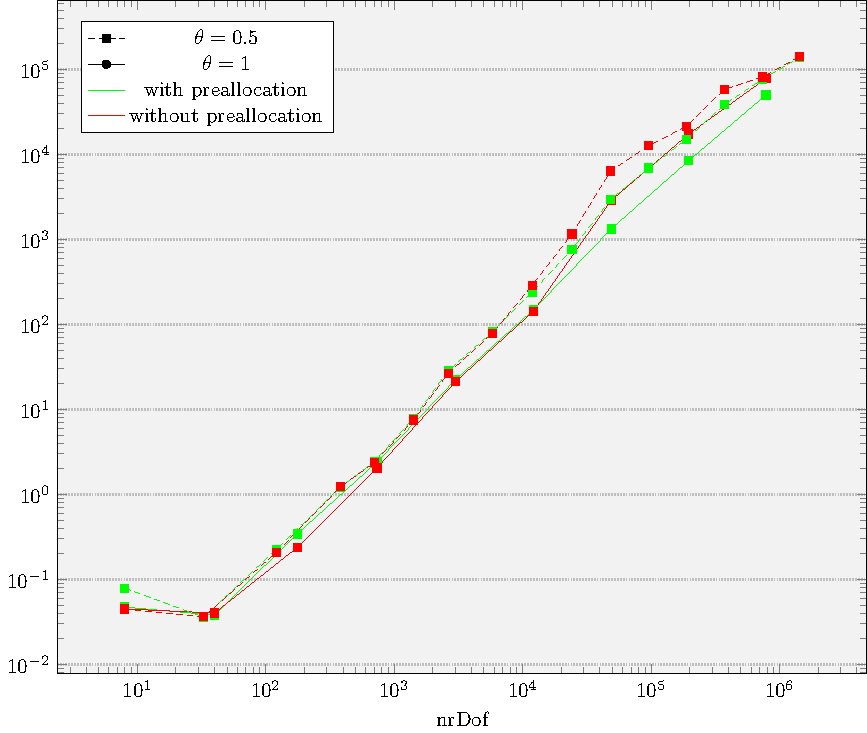
\includegraphics[width=0.8\linewidth]
      {pictures/experiments/appendix/timeCompPrealloc.pdf}
  \end{figure}
\end{frame}

\begin{frame}{Input Signal $f$, $\theta = 1$}
  \begin{figure}[!ht]
    \centering
    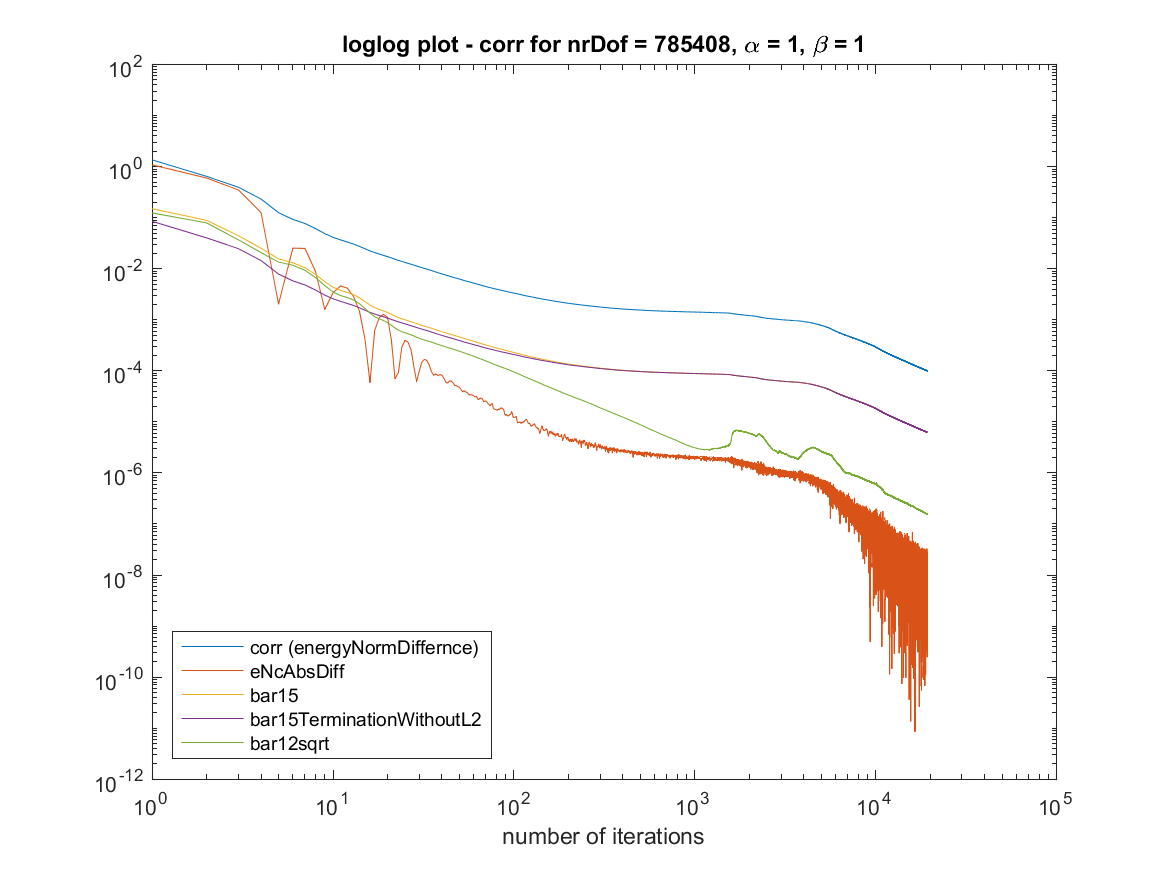
\includegraphics[width=0.9\linewidth]
      {pictures/experiments/appendix/f01UniformLvl8.png}
  \end{figure}
\end{frame}

\begin{frame}
  Let $u_P:[0,\infty)\to\Rbb$ with $u_P(r)=0$ for $r\geq 1$,
  and, for all $x\in\Omega$, $u(x)= u_P\big(|x|\big)$. 
  %\pause
  Furthermore, assume the existence  of $\partial_r u_P$ a.e.\ in $[0,\infty)$,
  the existence of the derivative of
  \begin{align*}
    \operatorname{sgn}\big(\partial_r u_P(r)\big)
    \coloneqq
    \begin{cases}
      -1 &\text{für }\partial_r u_P(r)<0,\\
      x\in[0,1] &\text{für }\partial_r u_P(r)=0,\\ 
      1 &\text{für }\partial_r u_P(r)>0.
    \end{cases}
  \end{align*}
  a.e.\ in $[0,\infty)$, and
  that $\operatorname{sgn}\big(\partial_r u_P(r)\big)/r\to 0$ as $r\to 0$.
  %\pause
  For all $r\in[0,\infty)$, define 
  \begin{align*}
    f_P(r)
    \coloneqq 
    \alpha u_P(r) - \partial_r\left(\operatorname{sgn}\big(\partial_r u_P(r)\big)\right) 
    - \frac{\operatorname{sgn}\big(\partial_r u_P(r)\big)}{r}
  \end{align*}
  %\pause
  Then $u$ solves the continuous problem
  on $\Omega\supseteq \left\{w\in\Rbb^2\,\middle|\, |w|\leq 1\right\}$ if
  the input signal is $f(x)\coloneqq f_P\big(|x|\big)$.
\end{frame}
